\PassOptionsToPackage{colorlinks,linkcolor={blue},citecolor={blue},urlcolor={blue},breaklinks=true,final}{hyperref}
\PassOptionsToPackage{dvipsnames}{xcolor}
\documentclass[xcolor={dvipsnames,svgnames},aspectratio=169]{beamer}

\usepackage{fontawesome5}
\usepackage{booktabs} % For better table formatting

\title{Concurrent Programming}
\subtitle{Week 8 (Lecture 1)}
\author{Stelios Tsampas}
\institute{
  \faEnvelope \; stelios@imada.sdu.dk
  \qquad
  \faGlobe \;
  \href{https://www.steliostsampas.com}{https://www.steliostsampas.com}
  \\\\\
  \faGithub \; stelios-tau/cp-2025
  \qquad\;\;
    \faDiscord \; cp-2025 (invite link in itslearning)
}
\date{February 17, 2025}

\titlegraphic{
\includegraphics[height=0.6cm,keepaspectratio]{../media/sdu-black.eps}}

\usetheme[block=fill]{metropolis}


%\usepackage{pres-common}
\usepackage{textpos}
\usepackage{centernot}

% \newcommand{\Goesv}[3]{\ensuremath{#1 \xRightarrow{~#3~} #2}}
% \newcommand{\goesv}[3]{\ensuremath{#1 \xrightarrow{~#3~} #2}}

% \usepackage{etex}
% \usepackage{semantic}

\usepackage[utf8]{inputenc}
\usepackage[english]{babel}
\usepackage{tikz}
\usepackage{hyperref}

\usetikzlibrary{arrows,shapes,matrix}
\usetikzlibrary{backgrounds}
\usetikzlibrary{positioning}
\usetikzlibrary{automata}
\usetikzlibrary{mindmap}
\usetikzlibrary{shapes.callouts}
\usetikzlibrary{decorations.text}
\usetikzlibrary{tikzmark}
\usetikzlibrary{calc}
\usetikzlibrary{overlay-beamer-styles}

\tikzset{onslide/.code args={<#1>#2}{%
    \only<#1>{\pgfkeysalso{#2}} % \pgfkeysalso doesn't change the path
  }}

\setbeamercolor{mygray}{bg=Gray!20}

\tikzset{temporal/.code args={<#1>#2#3#4}{%
    \temporal<#1>{\pgfkeysalso{#2}}{\pgfkeysalso{#3}}{\pgfkeysalso{#4}} % \pgfkeysalso doesn't change the path
  }}

\tikzstyle{highlight}=[fill=green!50]
\tikzstyle{hgreen}=[fill=green!20]
\tikzstyle{hred}=[fill=red!50]
\tikzstyle{hblue}=[fill=blue!50]
\tikzstyle{hgray}=[fill=gray!50]

\addtobeamertemplate{frametitle}{}{%
\begin{textblock*}{100mm}(\textwidth-2cm,-0.86cm)

\includegraphics[height=0.6cm,keepaspectratio]{../media/sdu-white.eps}
\end{textblock*}}

%\usepackage{tikz-cd}
% \usepackage{wasysym}
% \usepackage{color}
% \usepackage[matrix,arrow]{xy}
% \xyoption{all}
% \SelectTips{cm}{}
% % \usepackage{cite}
% \usepackage{amsthm}
% \usepackage{amsmath}
% \usepackage{bbold}
% % \usepackage[bbgreekl]{mathbbol}
% \usepackage{amssymb}
% \usepackage{pifont}
% \usepackage{mathtools}
% \usepackage{amsbsy}
% % \usepackage{paralist}
% \usepackage{shadethm}
% % \usepackage{fancyhdr}
% \usepackage{stmaryrd}
% \usepackage{wasysym}
% \usepackage{graphicx}
% \usepackage{tabularx}
% \usepackage{dsfont}
% \usepackage{ulem}




%\bibliography{mainBiblio}

%\includeonlyframes{current}
\begin{document}

\frame{\titlepage}

\def\firstcircle{(0,0) circle (2cm)}
\def\secondcircle{(1.4,1.4) circle (2cm)}
\def\thirdcircle{(0:2.4) circle (2cm)}

\begin{frame}[fragile]
  \frametitle{Teaching crew}

  \begin{columns}
    \begin{column}{0.33\textwidth}
      \begin{center}
        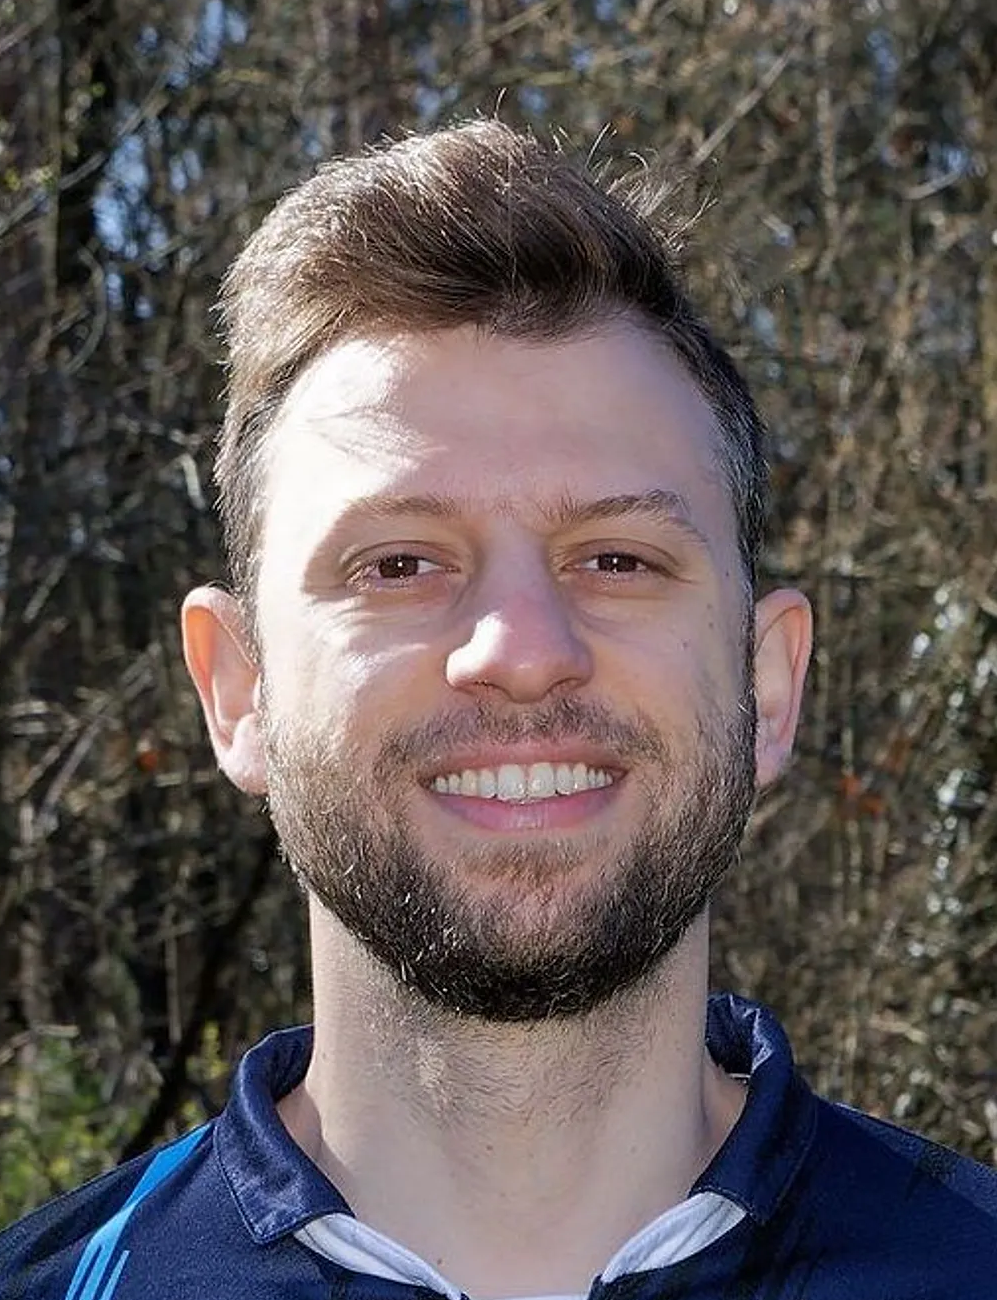
\includegraphics[height=3cm,keepaspectratio]{../media/stelios.png}
        \\
        Stelios Tsampas\\
        Responsible for DM584
        stelios@imada.sdu.dk
      \end{center}
    \end{column}
    \begin{column}{0.33\textwidth}
      \begin{center}
        
\includegraphics[height=3cm,keepaspectratio]{../media/jonas.png}
        \\
        Jonas Bork Jørgensen
        Instructor
        jonjo21@student.sdu.dk
      \end{center}
    \end{column}
    \begin{column}{0.33\textwidth}
      \begin{center}
        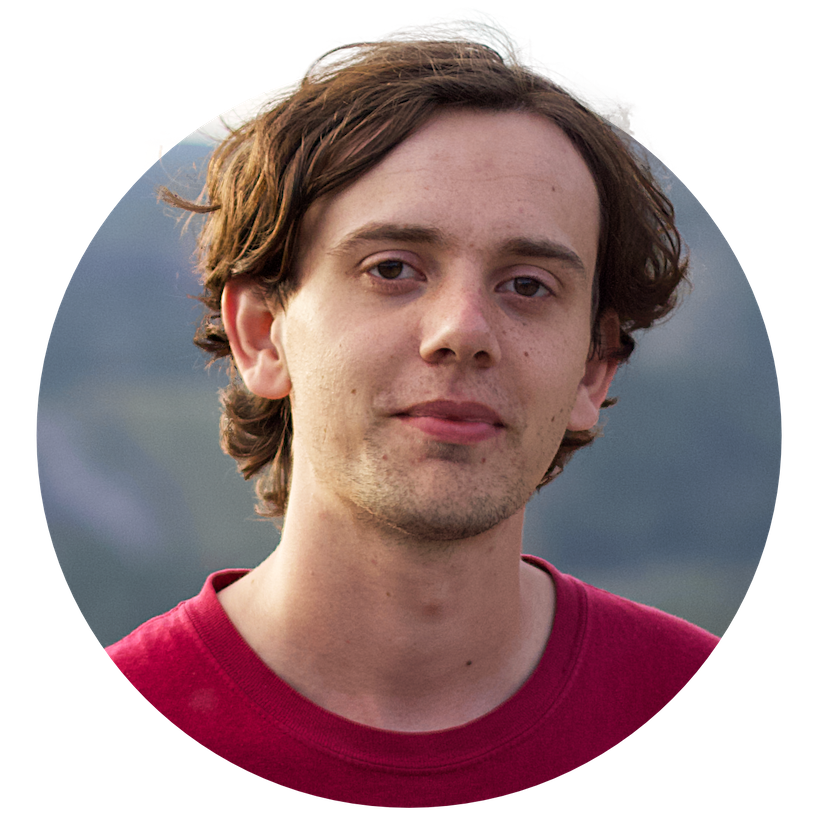
\includegraphics[height=3cm,keepaspectratio]{../media/viktor.png}
        \\
        Viktor Strate Kløvedal
        Instructor
        viktorstrate@imada.sdu.dk
      \end{center}
    \end{column}
  \end{columns}
  \vspace{0.6cm}
  Feel free to mail me, send me messages on Teams or Discord or drop by Ø14-602a-1.
\end{frame}

\begin{frame}{Outline}
  \tableofcontents
\end{frame}

\section{Overview}

\begin{frame}[fragile]
  \frametitle{Why Concurrent Programming?}

  \begin{itemize}
  \item[\faBook]<1-> Computers today have multi-core CPUs, and concurrency is essential for efficiency.
  \item[\faBook]<1-> Many applications (e.g., web servers, databases, operating systems) rely on handling multiple tasks at once.
  \item[\faBook]<1-> Understanding concurrency helps in writing efficient and
    bug-free programs.
  \end{itemize}
  \vspace{0.6cm}
  \uncover<2->{
  \begin{itemize}
  \item[\faSearch] Why do modern CPUs have more cores instead of just faster cores?
  \item[\faSearch] Why can a web server handle multiple users at once?
  \end{itemize}}
\end{frame}

\begin{frame}[fragile]
  \frametitle{What is concurrency?}

  \begin{block}{Concurrency}
    \emph{Concurrency} is the ability of a system to handle \textbf{multiple
      tasks}, seemingly \textbf{simultaneously}. These tasks may \textbf{not} execute at the
    exact same time, but their execution is \textbf{interleaved}.
  \end{block}

  \uncover<2->{
  \begin{itemize}
  \item[\faBook] Non-deterministic interleaving is the key characteristic.
  \item[\faBook] The programmer can make \textbf{no} assumptions as to the exact
    order of events.
  \item[\faSkullCrossbones] May involve \textbf{shared resources}, requiring
    synchronization.
  \end{itemize}
}
\onslide<3->{
  \begin{tikzpicture}[overlay, remember picture]
    \node[xshift=10cm,starburst,starburst points=25,
    align=center,fill=yellow, opacity=1,draw=red, line width=2pt]
    {\large{\textbf{Complete chaos!}}};
  \end{tikzpicture}}
\end{frame}

\begin{frame}[fragile]
  \frametitle{Concurrency is Hard!}

  \begin{itemize}
  \item[\faBook]<1-> Programming without concurrency is challenging already.
  \item[\faBook]<2-> It gets even harder when you have to think about threads of
    execution being executed together, interacting with one another.
  \item[\faBook]<3-> We can tackle this new challenge by equipping
    ourselves with:
    \begin{itemize}
    \item[\faCode]<3-> Clean programming principles, and
    \item[\faCode]<3-> Tools for concurrent programming.
    \end{itemize}
  \end{itemize}
\end{frame}

\begin{frame}[fragile]
  \frametitle{Overview of the course}

  \begin{itemize}
  \item[\faBook] Techniques for concurrent software.
  \item[\faJava] In Java!
  \item[\faBook] Key concepts of concurrency.
  \item[\faBook] Patterns and programming strategies for concurrency.
  \item[\faCode] Lots of practice and hands-on coding, both by me and you.
  \end{itemize}
\end{frame}

\begin{frame}[fragile]
  \frametitle{Course Structure}

  \begin{itemize}
  \item[\faBullhorn] Few of the lectures are taking place online through
    videos. Check itslearning to see which lectures are held in presence.
  \item[\faSchool] Links and videos will appear on itslearning.
  \item[\faGithub] The code for the lectures and the exercises is on GitHub.
  \item[\faBook] Book with theoretical aspects and code patterns.
  \item[\faCode] Exercises every week.
  \end{itemize}
\end{frame}

\begin{frame}[fragile]
  \frametitle{Main Book}
  \begin{columns}
    \begin{column}{0.5\textwidth}
      \begin{itemize}
      \item[\faBook] Java Concurrency in Practice, \emph{Briant Goetz et al.},
        Addison-Wesley, 2006.
      \item[\faGlobe] The book has a website, \href{http://jcip.net/}{http://jcip.net/}.
    \end{itemize}
    \end{column}
    \begin{column}{0.5\textwidth}  %%<--- here
      \begin{center}
        
\includegraphics[height=6cm,keepaspectratio]{../media/goetz-book.jpg}
      \end{center}
    \end{column}
  \end{columns}
\end{frame}

\begin{frame}[fragile]
  \frametitle{Chat and Q\&A}
  \begin{itemize}
  \item[\faDiscord] Join our discord server to chat with instructors and your
    colleagues.
  \item[\faDiscord] Entirely optional, link is in itslearning.
  \item[\faFileWord] I will also upload a link to a shared Word file to put all
    your questions in. Please use comments.
  \end{itemize}
\end{frame}

\begin{frame}[fragile]
  \frametitle{Exam}
  \begin{itemize}
  \item[\faGraduationCap] Software project (solo).
  \item[\faGraduationCap] You will all solve the same problem.
  \item[\faGraduationCap] Internal censor, 7-point scale.
  \item[\faGraduationCap] The problem will be given during the course.
  \end{itemize}
\end{frame}

\begin{frame}[fragile]
  \frametitle{Other considerations}
  \begin{itemize}
  \item[\faBook] Follow the content posted on itslearning.
  \item[\faBook] You can use whatever IDE/Code Editor that you like, both during the
    course and for developing the final software project, as long as you respect
    the final instructions for the exam when you hand in.
  \item[\faBook] The course consists of two main parts:
    \uncover<2->{
    \begin{itemize}
    \item[\faCode] Advanced Java, where we will cover some preliminaries about the Java
      language that are necessary for dealing well with concurrency.
    \item[\faCode] Concurrency, where we will deal with content specific to concurrency
      (principles, patterns, coding strategies).
    \end{itemize}}
  \end{itemize}
\end{frame}

\section{Concurrency 101}

\begin{frame}[fragile]
  \frametitle{Examples of Concurrency}

  Picture a chef (or more than one) cooking multiple dishes at the same time:

  \begin{itemize}
  \item[\faBook]<1-> The chef prepares multiple meals at once by switching tasks.
  \item[\faBook]<2-> They might chop vegetables, then stir a sauce, then check the oven.
  \item[\faBook]<3-> The dishes are interleaved but not truly parallel.
  \end{itemize}
\end{frame}

\begin{frame}[fragile]
  \frametitle{Case 1: one chef}

  \begin{center}
    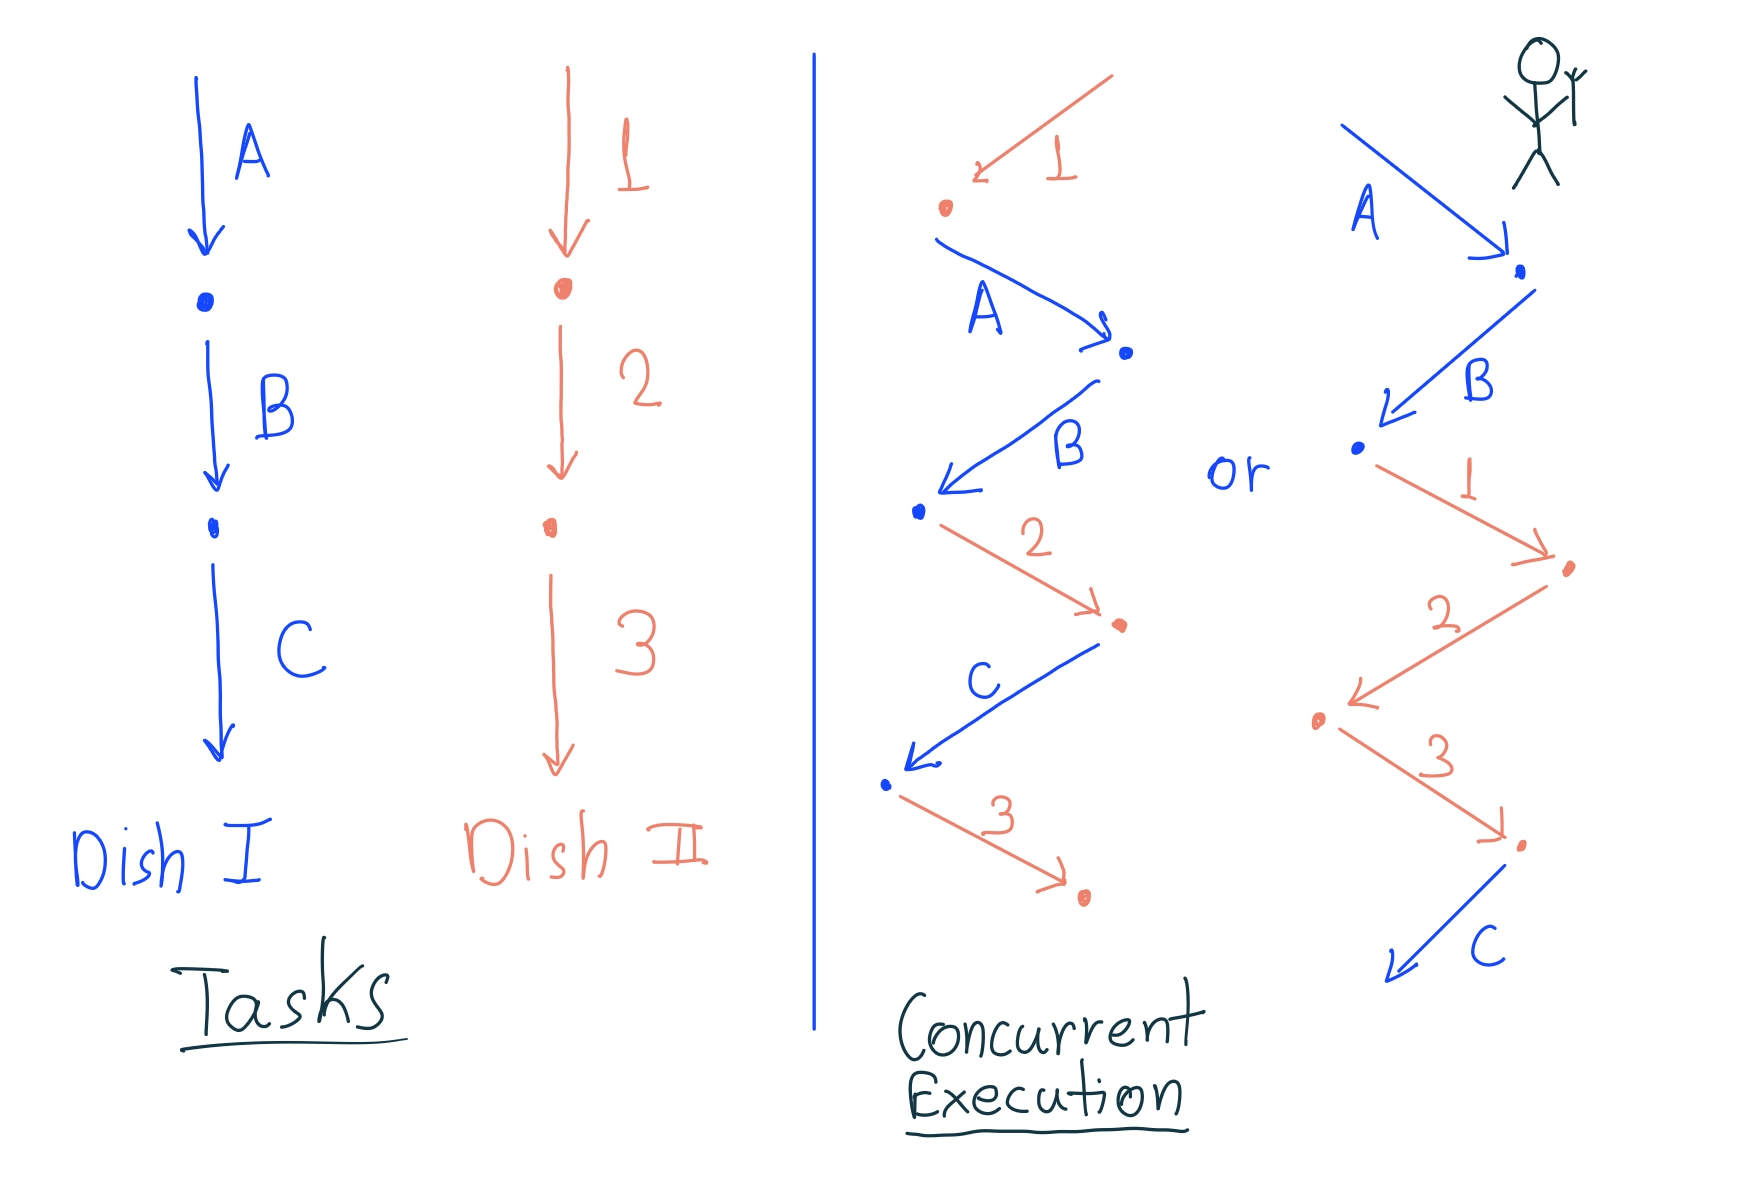
\includegraphics[width=11cm,keepaspectratio]{../media/lecture1-chef.png}
  \end{center}

  \onslide<2->{
    \begin{tikzpicture}[overlay, remember picture]
      \node[xshift=3cm,yshift=5cm,starburst,starburst points=30,
      align=center,fill=yellow, opacity=1,draw=red, line width=2pt]
      {\textbf{Nondeterministic \faSkullCrossbones}};
    \end{tikzpicture}}

\end{frame}

\begin{frame}[fragile]
  \frametitle{Case 1: one chef}

  \large{
  \begin{itemize}
  \item[\faBook]<1-> You don't need more than one chef/CPU cores/threads to have
    concurrent execution.
  \item[\faBook]<1-> \textbf{Task switching}/\textbf{interleaving} are the hallmarks of
    concurrency.
  \end{itemize}}
\end{frame}

\begin{frame}[fragile]
  \frametitle{Degenerate (non-)example, sequential execution}

  \begin{center}
    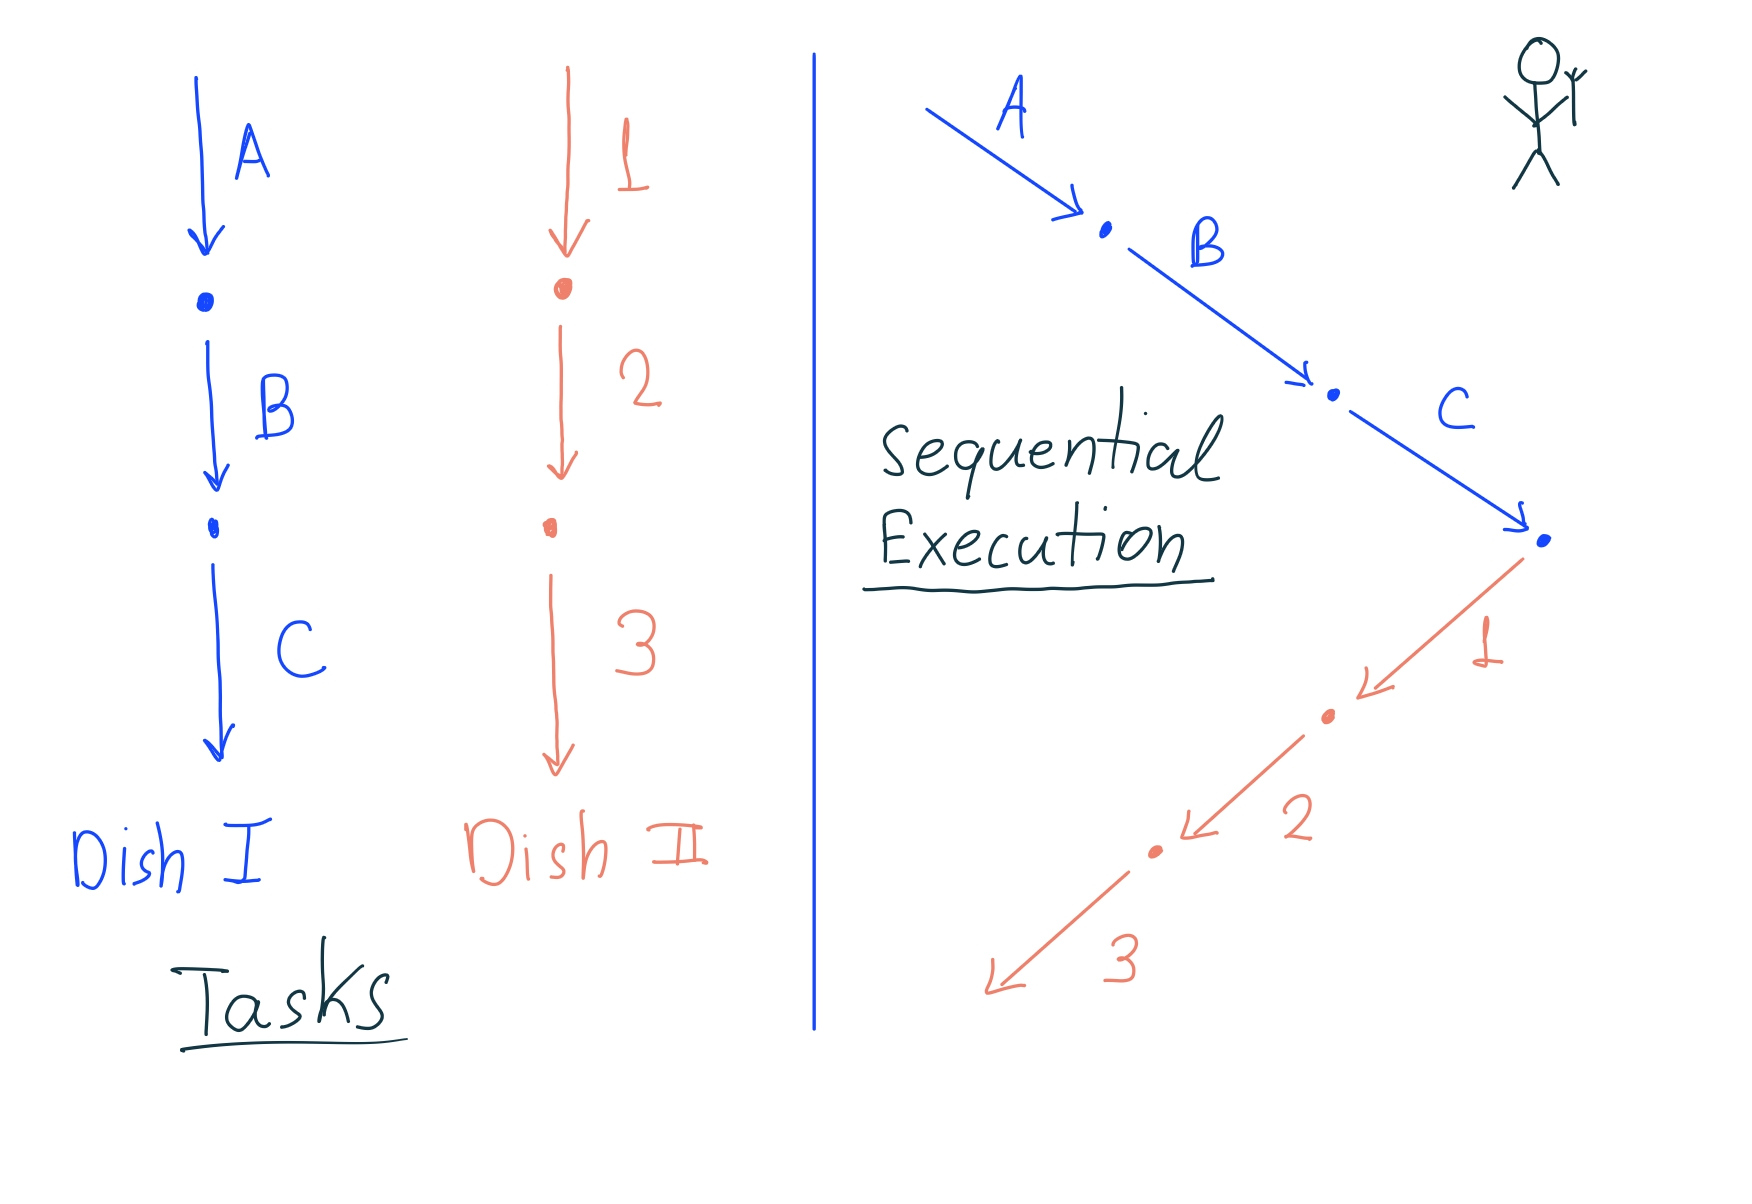
\includegraphics[width=11cm,keepaspectratio]{../media/lecture1-seq.png}
  \end{center}

  \onslide<2->{
    \begin{tikzpicture}[overlay, remember picture]
      \node[xshift=3cm,yshift=5cm,ellipse,
      align=center,fill=green!20, opacity=1,draw=black, line width=0.4pt]
      {\textbf{Predictable \faCheck}};
    \end{tikzpicture}}

\end{frame}

\begin{frame}[fragile]
  \frametitle{Degenerate (non-)example, sequential execution}

  \large{
    \begin{itemize}
    \item[\faBook]<1-> In sequential execution, tasks are \emph{sequenced},
      their execution will not be interrupted.
    \item[\faBook]<2-> Simple and predictable, the kind of programming you have
      been doing so far.
    \end{itemize}}

\end{frame}


\begin{frame}[fragile]
  \frametitle{Case 2: two chefs}

  \begin{center}
    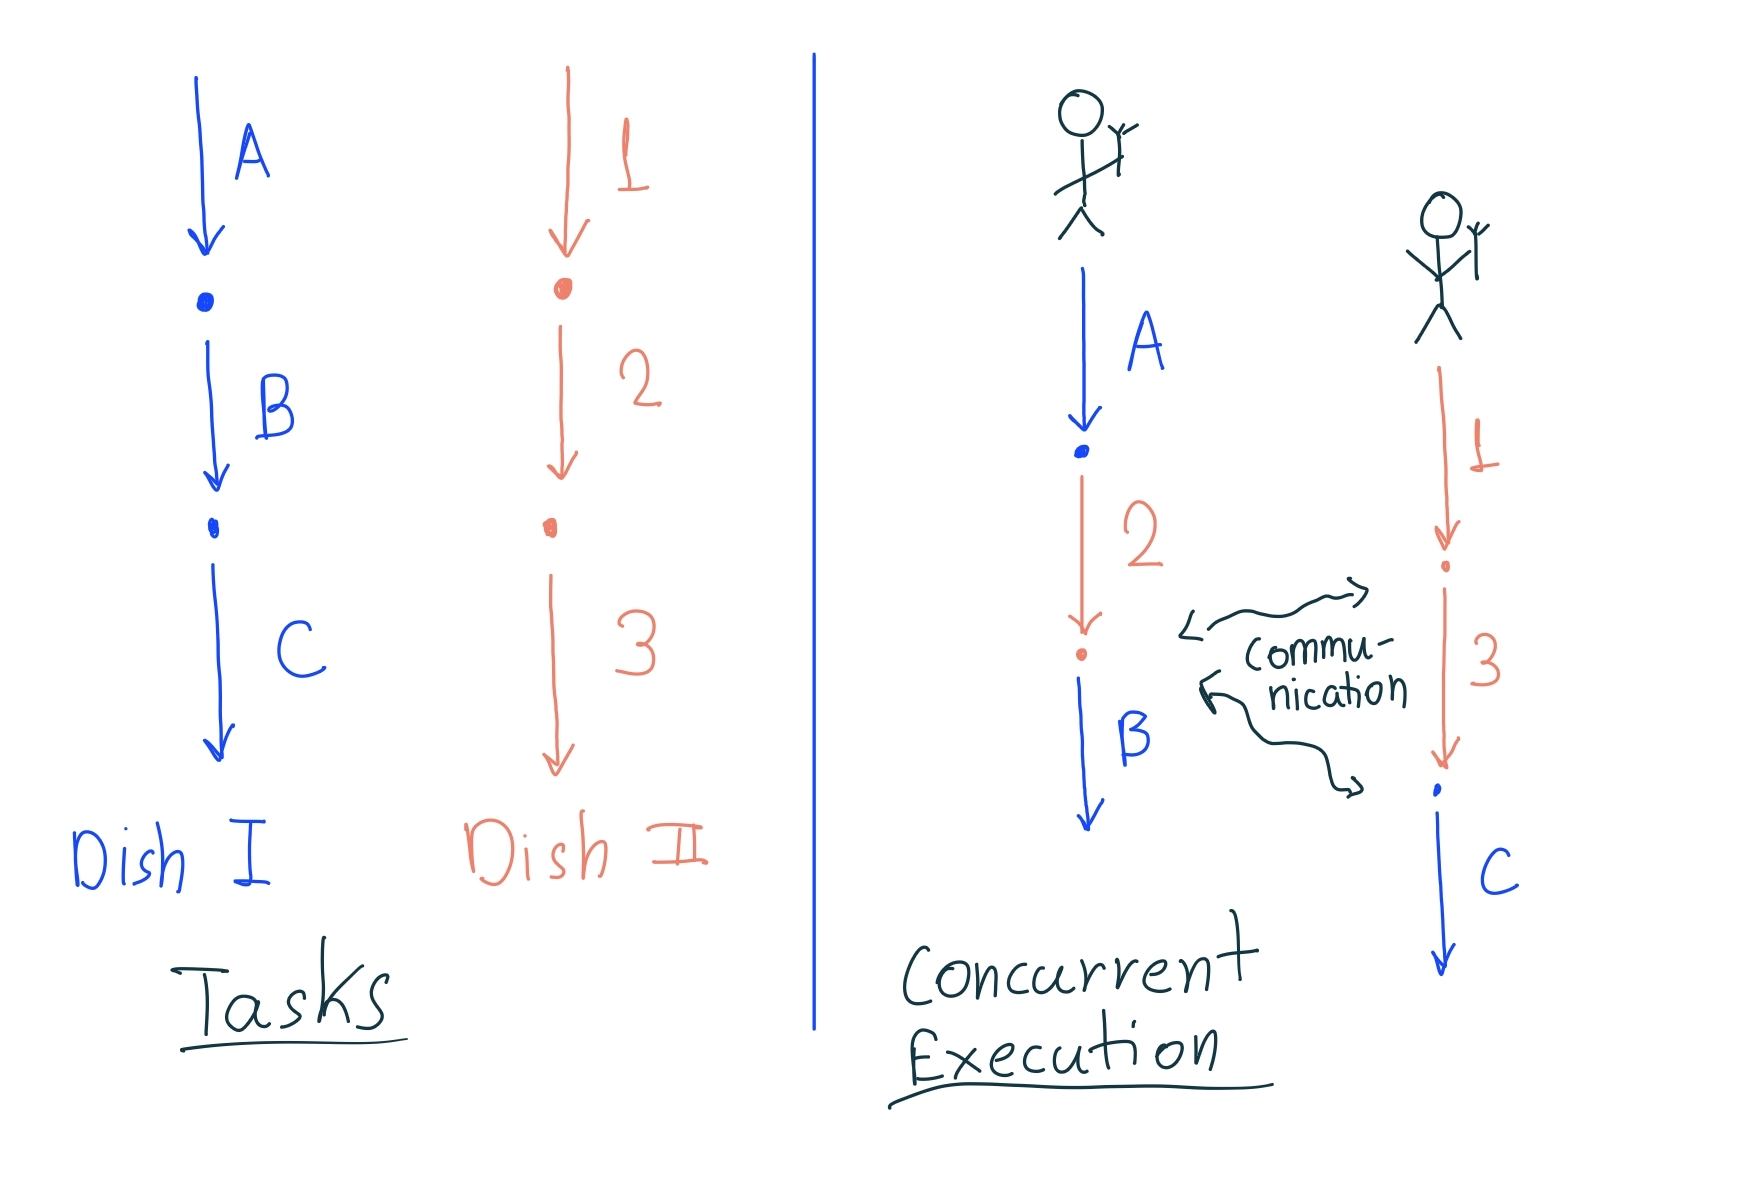
\includegraphics[width=11cm,keepaspectratio]{../media/lecture1-twochefs.png}
  \end{center}

  \onslide<2->{
    \begin{tikzpicture}[overlay, remember picture]
      \node[xshift=3cm,yshift=5cm,starburst,starburst points=30,
      align=center,fill=yellow, opacity=1,draw=red, line width=2pt]
      {\textbf{Nondeterministic \faSkullCrossbones}};
    \end{tikzpicture}}
\end{frame}

\begin{frame}[fragile]
  \frametitle{Case 2: two chefs}

  \large{
    \begin{itemize}
    \item[\faBook]<1-> This time there are actually distinct chefs/\textbf{threads} of
      execution taking place.
    \item[\faBook]<2-> They might be sharing resources (i.e. using the same
      equipment, food), so extra care needs to be taken, especially because the
      interleaving is \textbf{non-deterministic}.
    \item[\faBook]<3-> Remember that these \textbf{threads} are abstractions, it
      is not necessary that, underneath the surface, their a multi-core CPU
      executing each thread.
    \end{itemize}}
\end{frame}

\begin{frame}[fragile]
  \frametitle{Degenerate (non-)example 2, parallelism}

  \begin{center}
    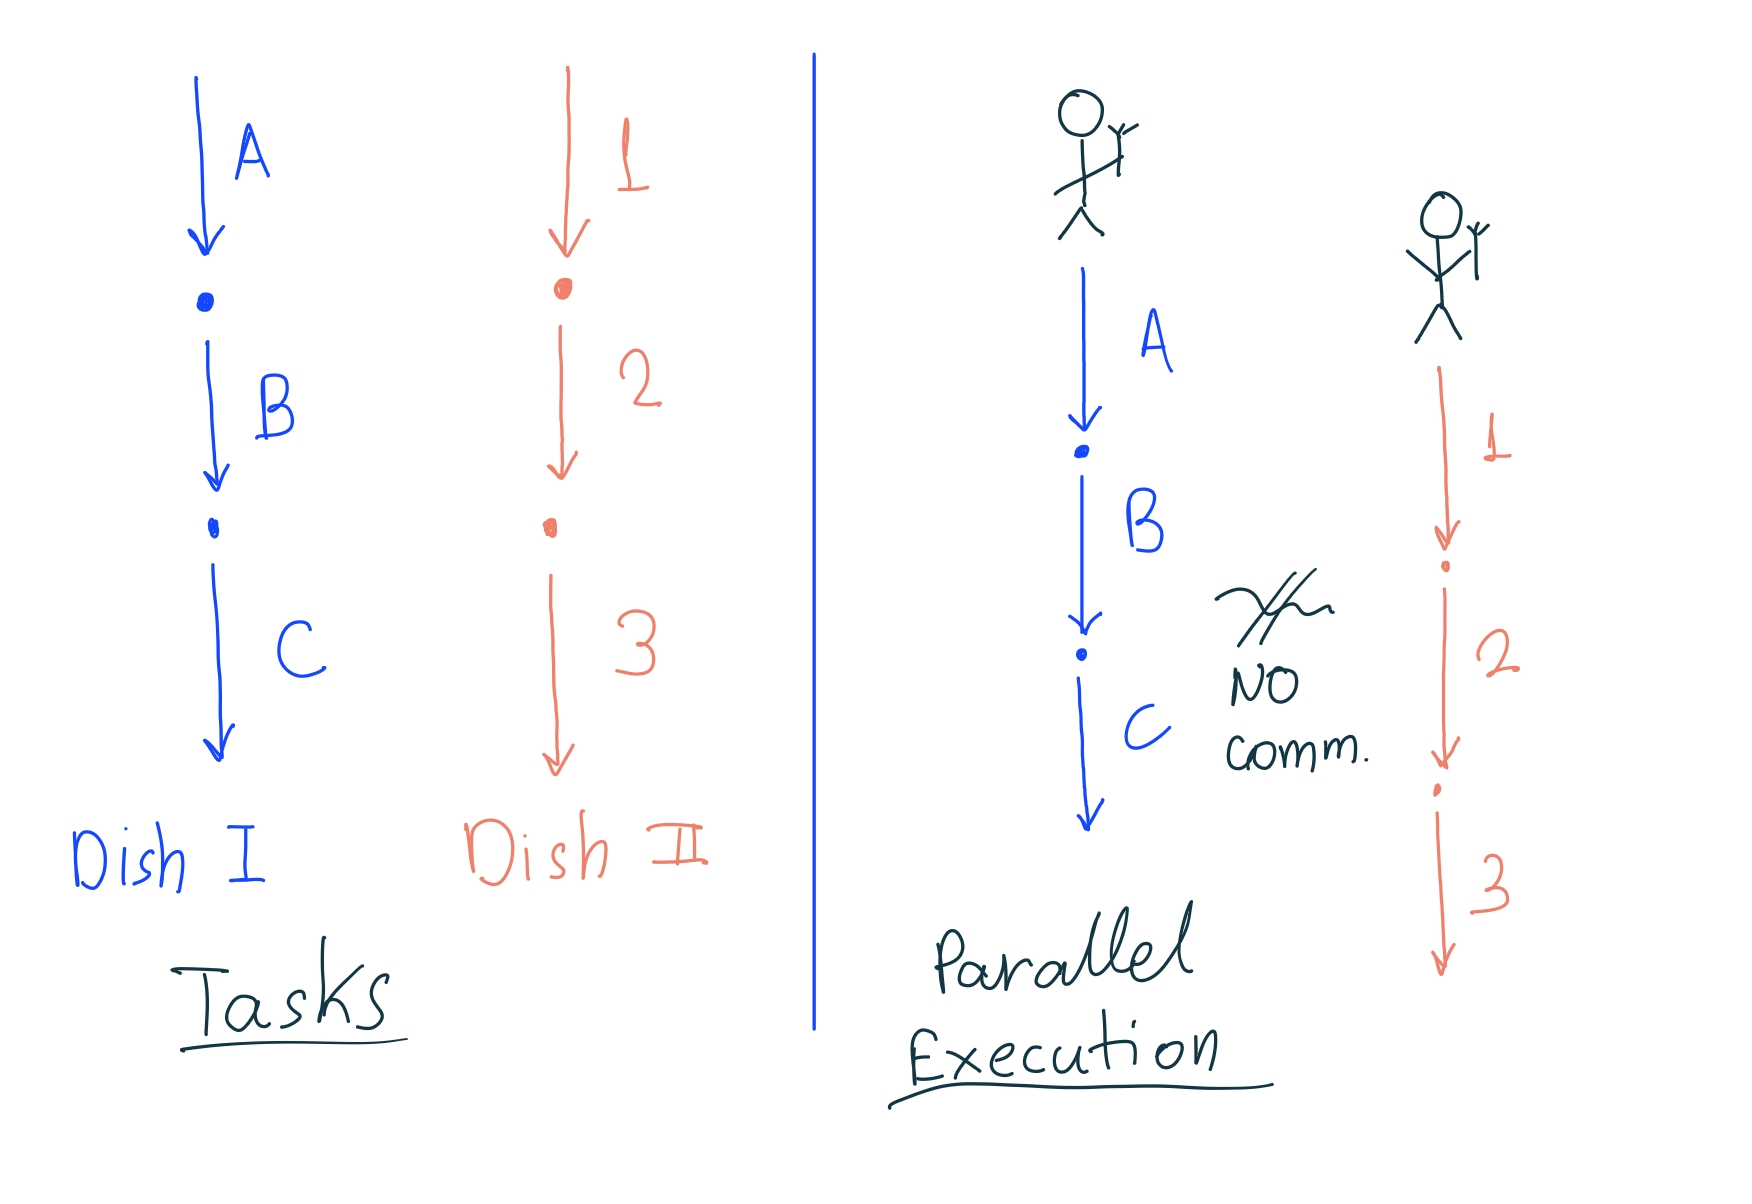
\includegraphics[width=11cm,keepaspectratio]{../media/lecture1-para.png}
  \end{center}

  \onslide<2->{
    \begin{tikzpicture}[overlay, remember picture]
      \node[xshift=3cm,yshift=5cm,ellipse,
      align=center,fill=green!20, opacity=1,draw=black, line width=0.4pt]
      {\textbf{Predictable \faCheck}};
    \end{tikzpicture}}
\end{frame}

\begin{frame}[fragile]
  \frametitle{Degenerate (non-)example 2, parallelism}

  \large{
    \begin{itemize}
    \item[\faBook]<1-> Again, there are two chefs/\textbf{threads} of
      execution taking place.
    \item[\faBook]<1-> However, their tasks are distinct, and there is no
      communication between the two.
    \item[\faBook]<1-> This is \textbf{parallel programming}, a different topic
      that is about the developing algorithms that make use of
      multiple CPU units.
    \item[\faBook]<2-> \textbf{Not} quite the topic of this class,
      although the programming techniques involved may overlap.
    \end{itemize}}

\end{frame}

\begin{frame}{Key Differences: Concurrency vs. Parallelism}
  \vspace{-0.4cm}
\begin{table}[]
    \centering
    \begin{tabular}{l|l|l}
        \toprule
      \textbf{Feature}
      & \textbf{Concurrency}
      & \textbf{Parallelism} \\
        \midrule
      \textbf{Definition}
      & Interleaved execution
      & True simultaneous execution\\
        \midrule
      \textbf{Execution}
      & Task switching, may be single-core
      & Requires multiple cores \\
        \midrule
      \textbf{Use Case}
      & Responsiveness (UI, servers)
      & Performance (big data, heavy comp.) \\
        \midrule
      \textbf{Hardware}
      & Can work on single-core
      & Requires multi-core CPU \\
        \midrule
      \textbf{Example}
      & Multi-threading with task switching
      & Multi-threading with multiple cores \\
        \midrule
      \textbf{Java}
      & \texttt{Thread}, \texttt{ExecutorService}
      & \texttt{ForkJoinPool}, \texttt{parallelStream()} \\
      \midrule
      \textbf{Resources}
      & Shared resources, synchronization
      & Little to no sharing and communication\\
      \midrule
      \textbf{Effect}
      & Non-deterministic
      & (Largely) deterministic\\
        \bottomrule
    \end{tabular}
  \end{table}
  \onslide<3->{
    \begin{tikzpicture}[overlay, remember picture]
      \node[xshift=4cm,yshift=3cm,starburst,starburst points=25,
      align=center,fill=yellow, opacity=1,draw=red, line width=2pt]
      {\large{\textbf{Complete chaos!}}};
    \end{tikzpicture}
    \begin{tikzpicture}[overlay, remember picture]
      \node[xshift=11cm,yshift=3cm,ellipse,
      align=center,fill=green!20, opacity=1,draw=black, line width=0.4pt]
      {\large{\textbf{Predictable \faCheck}}};
    \end{tikzpicture}}
\end{frame}

% \begin{frame}[fragile]
%   \frametitle{What is concurrency?}

%   \begin{block}{Concurrency}
%     \emph{Concurrency} is the ability of a system to handle \textbf{multiple
%       tasks}, seeminly \textbf{simultaneously}. These tasks may \textbf{not} execute at the
%     exact same time, but their execution is \textbf{interleaved}.
%   \end{block}

%   \begin{itemize}
%   \item[\faBook] Non-deterministic interleaving is the key characteristic.
%   \item[\faBook] The programmer can make \textbf{no} assumptions as to the exact
%     order of events.
%   \item[\faSkullCrossbones] May involve \textbf{shared resources}, requiring
%     synchronization.
%   \end{itemize}
%   \onslide<2->{
%     \begin{tikzpicture}[overlay, remember picture]
%       \node[xshift=10cm,starburst,starburst points=25,
%       align=center,fill=yellow, opacity=1,draw=red, line width=2pt]
%       {\textbf{Complete chaos!}};
%     \end{tikzpicture}}
% \end{frame}

% \begin{frame}[fragile]
%   \frametitle{Why bother then?}

%   \begin{itemize}
%   \item[\faBook] Improves responsiveness (e.g., UI remains interactive).
%   \item[\faBook] Utilizes multi-core processors for performance gains.
%   \item[\faBook] Handles multiple tasks efficiently (e.g., web servers
%     processing multiple requests)
%   \end{itemize}
% \end{frame}

\begin{frame}[fragile]
  \frametitle{What this is all about}

  \large{A large amount of this class is about managing the \textbf{sharing} of resources
  and generally the \textbf{communication} and \textbf{coordination} of these
  \textbf{threads} of execution. \uncover<2->{Yes, the term \emph{threads} is
    the technically correct term.}}
\end{frame}

\begin{frame}[fragile]
  \frametitle{Threads}

  \begin{itemize}
  \item[\faBook] The main abstraction that is involved in concurrency.
  \item[\faBook] A thread represents a lightweight, independent unit of
    execution.
  \item[\faBook] Threads are present at multiple levels of the
    software stack:
    \begin{itemize}
    \item[\faLinux] Operating system level, i.e. user and kernel threads.
    \item[\faCode] At the level of programming languages, Java threads, pthreads
      in C...
    \end{itemize}
  \item[\faBook] There can be many active threads active at the same time, i.e.
    \emph{concurrently}.
  \item[\faExclamation]<2-> ... but they do not need to run at the actual same moment.
  \end{itemize}
\end{frame}

\begin{frame}[fragile]
  \frametitle{Threads vs processes}

  \begin{center}
    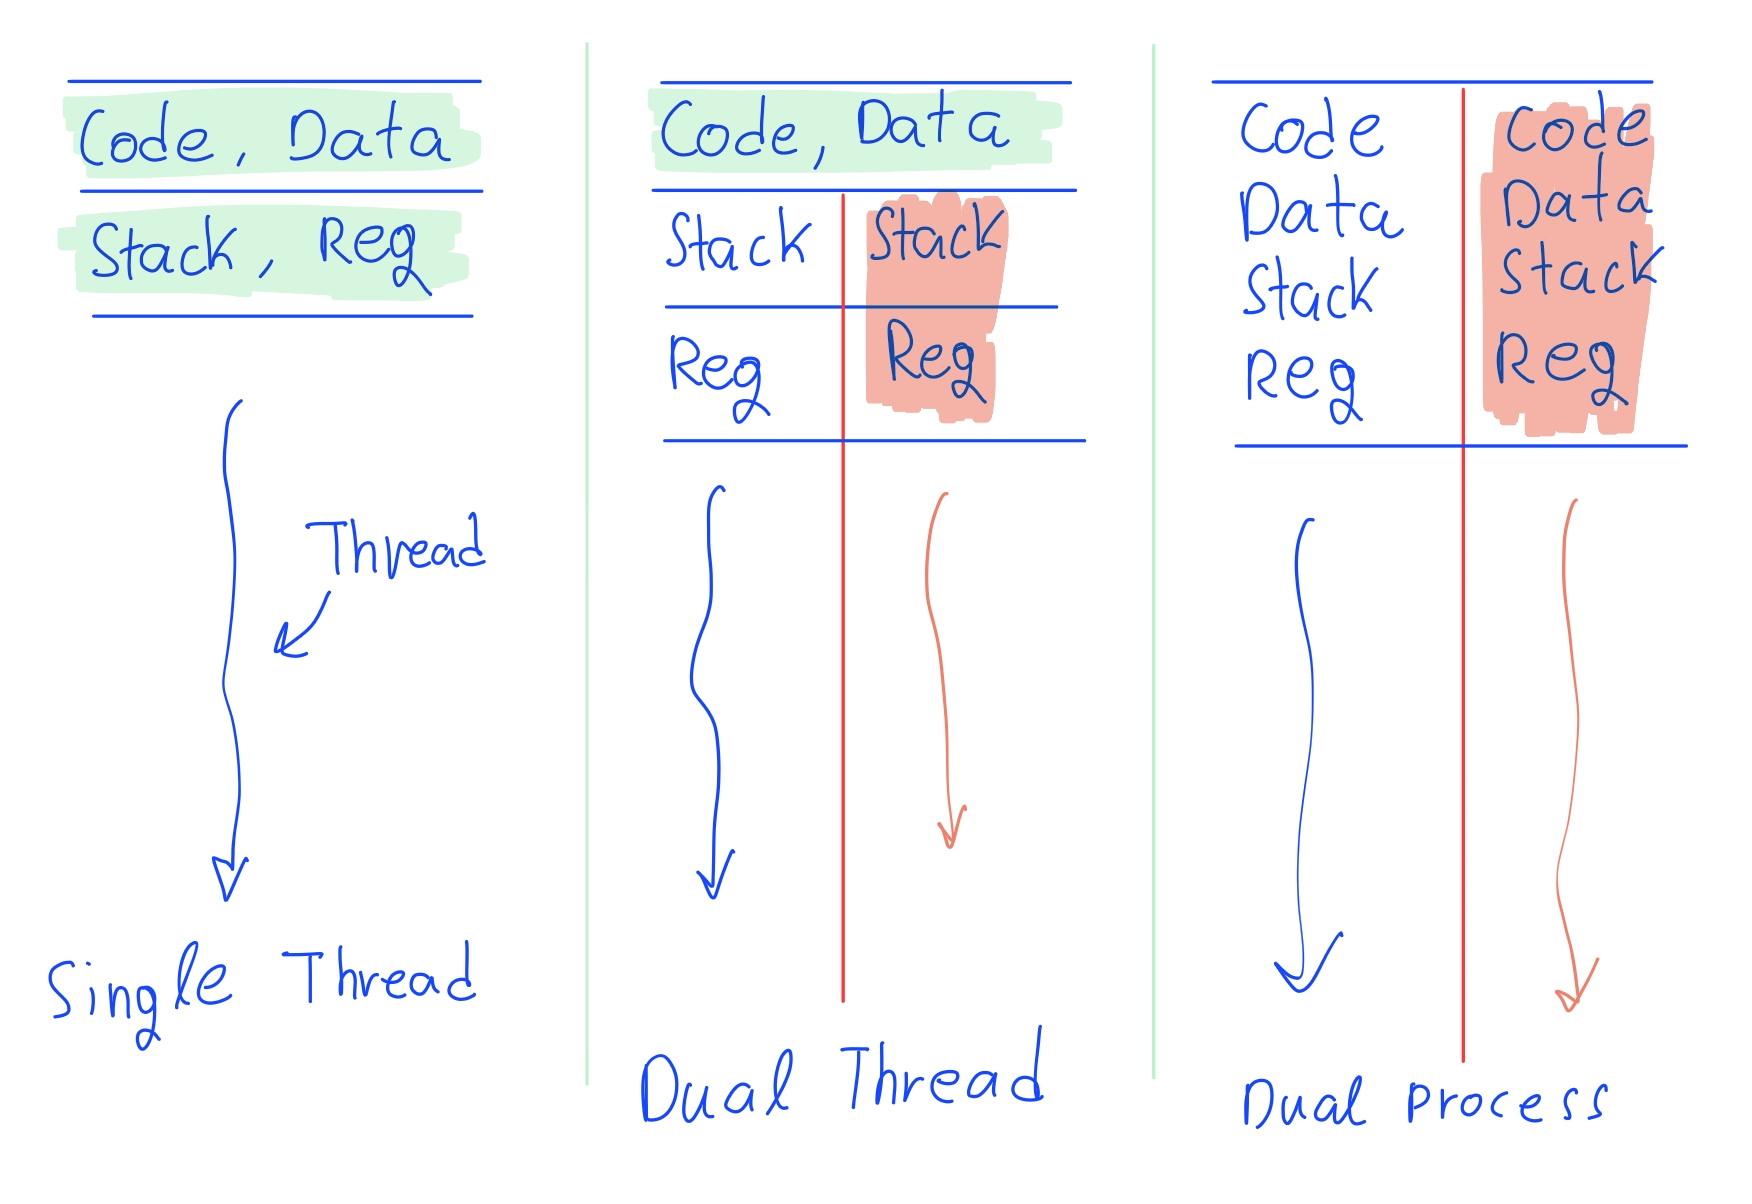
\includegraphics[width=11cm,keepaspectratio]{../media/lecture1-threads.png}
  \end{center}

\end{frame}

\begin{frame}[fragile]
  \frametitle{Dangerous pitfalls (will be dealing a lot with those)}

  \begin{itemize}
  \item[\faUserInjured] \textbf{Race conditions}: Multiple threads accessing and
    modifying shared data inconsistently.
    \begin{itemize}
    \item[\faBriefcaseMedical]<2-> Proper, careful synchronization.
    \end{itemize}
  \item[\faUserInjured] \textbf{Deadlocks}: Threads waiting indefinitely for each
    other.
    \begin{itemize}
    \item[\faBriefcaseMedical]<2-> Proper, careful synchronization.
    \end{itemize}
  \item[\faUserInjured] \textbf{Starvation}: Some threads never get CPU time due to
    scheduling.
    \begin{itemize}
    \item[\faBriefcaseMedical]<2-> Proper, careful synchronization.
    \end{itemize}
  \item[\faUserInjured] \textbf{Visibility Issues}: Changes in one thread
    not visible to others.
    \begin{itemize}
    \item[\faBriefcaseMedical]<2-> Make no assumptions on data sharing between threads.
    \end{itemize}
  \end{itemize}
\end{frame}

% \section{Course Schedule}

\begin{frame}{}
  \centering \huge
  Thank you!
\end{frame}

% \begin{frame}[allowframebreaks]
%   \frametitle{Bibliography}
%   \printbibliography
% \end{frame}

\end{document}

%%% Local Variables:
%%% mode: latex
%%% TeX-engine: xetex
%%% TeX-master: t
%%% End:
